For each of the afforementioned passages the throughflow was computed. This is done using a simple integration to calculate the volumetric flux through each passage.
\begin{align}
	Q = \int \int_A \vec{u} \cdot d\vec{A}
\end{align}	
For each passage a suitible location was chosen such that there are no boundaries next to the passageways. Then the $u$ component of the flow is used to compute the total flow. This method is the same for each of the passages and thus we can study the effect of changes in bathymetry to on the relative strenght of the flow. However, it should be noted that these values may not represent real physical values. As the passages are often only a few gridcells wide and, the nature of the 4 degree model. Resulting in discepencies due to boundary conditions. The passageways have been labeled in figure (figure of these) and results are plotted in figure (figure of these).

%\begin{figure}[H]
%	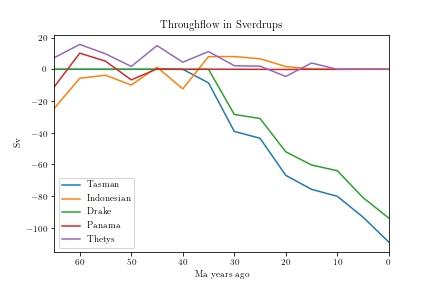
\includegraphics[width=\linewidth]{throughflow}
%	\caption{test caption}
%	\label{fig:throughflow}
%\end{figure}

There is still some uncertanty in the method of calculating the throughflow. The method used in \fref{fig:throughflow} is calculated using the velocity field. Another method is using the Barotropic stream function discussed in \fref{sec:BSF}. The stream fuction $\Psi'$ is defined by


$$
u = \frac{\partial \Psi'}{\partial y}, v = \frac{\partial \Psi'}{\partial x}
$$

In veros it is computed by integrating the barotropic flow from north to south. This gives values for the volumetric flow of each gridcell. Where a positive value indicates clockwise flow and a negative value anticlockwise flow. This can thus also be used as a measure of the throughflow for each passage. These values are given in (figure)

As is visible, these values are quite diffirent that the values obtained in \fref{fig:throughflow}.
They give an image of a much weaker flow. This can probably be attributed to the fact that interpolation is used at the coasts. resulting in the barotropic streamfunction being zero on the boundary of some coasts.


To get a better understanding of the flows we can look at a vector field showing the direction of horizontal water displacement. This is done by making a weighted mean of the horizontal flow field for each layer. Weighted by the volume of each grid cell. In this way each arrow actually represents relative flow velocity compared to other grid points.

This field is shown in figure ...

%TODO add figure of flow

The flow field clearly shows that...